\documentclass[10pt]{beamer}

\usetheme{metropolis}
\usepackage{appendixnumberbeamer}

\usepackage{booktabs}
\usepackage[scale=2]{ccicons}

\usepackage{pgfplots}
\usepgfplotslibrary{dateplot}

\usepackage{xspace}

\usepackage{tikz}
	\usetikzlibrary{shapes.geometric, arrows, positioning}
	\tikzstyle{startstop} = [rectangle, rounded corners, minimum width=3cm, minimum 		height=1cm,text centered, draw=black, fill=red!30]
	\tikzstyle{io} = [trapezium, trapezium left angle=70, trapezium right angle=110, minimum width=3cm, minimum height=1cm, text centered, draw=black, fill=blue!30]
	\tikzstyle{process} = [rectangle, minimum width=3cm, minimum height=1cm, text centered, draw=black, fill=orange!30]
\tikzstyle{decision} = [diamond, minimum width=3cm, minimum height=1cm, text centered, draw=black, fill=green!30]
\tikzstyle{arrow} = [thick,->,>=stealth]
\tikzstyle{arrow} = [thick,->,>=stealth]
%\usepackage{listings}
\usepackage{minted}

\usepackage{bm}%................................. Bold math symbols (after fonts)

\setbeamercolor{normal text}{bg=white}





\title{EML4930/EML6934: Lecture 09}
\subtitle{Reading, writing, and modifying text and CSV files in Python }
\date{October 26, 2017}
%\author{CJ}
\author{Charles Jekel}
%\titlegraphic{\includegraphics{images/avatarCropped.png}\vspace{58cm}}
%\institute{1. University of Florida\\ 2. Stellenbosch University, South Africa}

% \titlegraphic{\hfill\includegraphics[height=1.5cm]{logo.pdf}}

\begin{document}

\maketitle

\begin{frame}{Reminder: Quiz at the end of next class (11/02/2017)}
\begin{itemize}
\item Quiz will cover anything from lecture 00 - lecture 05
\item You should be able to write the code to plot a curve in Python from memory!
\item Sample quiz questions will be posted
\item I view lectures 00 - 05 as the basics of Python (these are the lectures the final exam will be about! + this lecture for reading and writing files) Lectures 06 - 13 build upon these basics for advanced cases. 
\end{itemize}
\end{frame}

\begin{frame}{Let's take a look at HW 09}
\begin{itemize}
\item You are presented with a practical structural optimization problem
\item You must create a couple functions to aid in the optimization
\item One function will take read an input template and write a modified version of the file
\item The other function reads specific values from a large output file
\item This HW is to prepare you for \textit{black-box} optimization (think of the input template and output file your results from some expensive simulation that you'll be running!)
\end{itemize}
\end{frame}

\begin{frame}{Topics for today's lecture}
\url{https://docs.python.org/3/tutorial/inputoutput.html}
\begin{itemize}
\item with statement
\item open function
\item methods for file objects
\item read file line by line
\item string manipulation
\item itertools islice efficient loops
\item read a csv file
\item write a csv file
\end{itemize}
\end{frame}

\begin{frame}{I've created a demo.txt file which contains the following}
This is line 1 of a demo txt file. 

This is line 2 of a demo txt file. 

This is line 3 of a demo txt file. 

This is line 4 of a demo txt file.

This is line 5 of a demo txt file.

This is line 6 of a demo txt file.

This is line 7 of a demo txt file.

This is line 8 of a demo txt file.

This is line 9 of a demo txt file.

This is line 10 of a demo txt file.

I replace\_me\_1 Python.

I replace\_me\_2 MATLAB.
\end{frame}

\begin{frame}[fragile]{The open() function in Python to load files.}
open() returns a file object as is most commonly used as 

\mint{python}|open(filename, mode)|

The following code will create a file object f by reading demo.txt.
\mint{python}|f = open('demo.txt', 'r')|

Typically the file object are opened in text mode, which means that you work with Python strings. 
\end{frame}

\begin{frame}{modes for open() text files}
\begin{table}
\begin{tabular}{ll}
\textbf{Mode} & \textbf{Description}  \\
\hline
'r' &	open file read only \\
 &	open file read only (assumed if left blank) \\
'w' & 	open file for writing only (existing files will be erased) \\
'a' &   open file for appending (data is written at the end of file) \\
'r+'&   open file for both reading and writing
\end{tabular}
\end{table}
\end{frame}

\begin{frame}{Unix and Windows end statements - text mode}
\begin{itemize}
\item Each line in the file object will have some kind of end line statement
\item a Windows file with have an end of string statement that looks like '\textbackslash r \textbackslash n'
\item Unix file will have an end of string statement that looks like '\textbackslash n'
\item these statements indicate where on the text file does a new line begin
\item When writing files Python automatically specifies platform dependent line endings.
\end{itemize}
\end{frame}

\begin{frame}{modes for open() binary files}
\begin{table}
\begin{tabular}{ll}
\textbf{Mode} & \textbf{Description}  \\
\hline
'rb' &	open file read only \\
'b' &	open file read only (assumed if left blank) \\
'wb' & 	open file for writing only (existing files will be erased) \\
'ab' &   open file for appending (data is written at the end of file) \\
'r+b'&   open file for both reading and writing
\end{tabular}
\end{table}
\end{frame}

\begin{frame}[fragile]{use .close() to close a file}
Let's say you opened demo.txt as
\mint{python}|f = open('demo.txt', 'r')|
The file will stay open (eating memory) until you explicitly close it. 

If you don't explicitly close a file, Python's garbage collection will eventually destroy the object and close the file for you. This is dangerous because it won't be consistent!

To close the text file we run
\mint{python}|f.close()|
\end{frame}

\begin{frame}{open() and .close() in summary}
\begin{itemize}
\item use open(filename, mode)
\item by default files are opened in text mode
\item you can also open binary files
\item use .close() to close a file
\end{itemize}
\end{frame}

\begin{frame}{Now that I've shown you open() and .close()}
\textbf{Never ever use open() and .close().}

It's bad to forget to close a file. So bad that you should never use open(). Rather we will be using the with statement which closes files automatically! 
\end{frame}

\begin{frame}{Let's take a look at the with statement}
What is a with statement? 

\url{https://docs.python.org/3/reference/compound\_stmts.html\#with}

The with statement is used to wrap the execution of a block with methods defined by a context manager (see section With Statement Context Managers). This allows common try-except-finally usage patterns to be encapsulated for convenient reuse.
\end{frame}

\begin{frame}[fragile]{How to open a file: use a with statement}
\begin{minted}
{python}
# start a with statement, this opens the 
with open('demo.txt', 'r') as f:
    # let's read the text data
    read_data = f.read()
    # let's print the read data
    print(read_data)
# once the indent is removed, the file is closed
# f is no longer in memory!, though read_data is
\end{minted}
\end{frame}

\begin{frame}{methods of file objects}
\begin{table}
\begin{tabular}{ll}
\textbf{Method} & \textbf{Description}  \\
\hline
.read() & return the entire contexts of a file as a single string \\
.read(size) & returns the contexts of your file for specified size \\
.readline() & reads a single line from the file (iterator) \\
.readlines() & read the entire file as a list, where each line is list item \\
.write(string) & write the string to the file (requires write mode) \\
.tell() & returns an integer indicating the current position in f \\
.seek(off,from) & go to some integer offset in file , from is either 1,2,or 3 \\
\end{tabular}
\end{table}
\textbf{Note}: The end of a file will be indicated by an empty string '', however a blank line will contain '\textbackslash n'.
\end{frame}

\begin{frame}[fragile]{Reading a file line by line is easy in Python}
For reading lines from a file, you can loop over the file object. This is memory efficient, fast, and leads to simple code:
\begin{minted}
{python}
with open('demo.txt', 'r') as f:
    for line in f:
        print(line)
\end{minted}
\end{frame}

\begin{frame}[fragile]{Methods for string manipulation - join}
Remember how I said strings were really objects long ago?

Let's pretend we have some list of strings
\mint{python}|data = ['a', 'b', 'c', 'd']|

we can use .join() to make a single string containing all of the strings 
\mint{python}|data_flat_string = ''.join(data)|

\mint{python}|print(data_flat_string)|
will return a single string of 'abcd'
\end{frame}

\begin{frame}[fragile]{Methods for string manipulation - split }
We can use the .split(string\_separator) to break a string into a list of strings, separated by string\_separator

Example: break up the string wherever there is a space
\begin{minted}
{python}
a = 'This is line 4 of a demo txt file.'
b = a.split(' ')
print(b)
\end{minted}
b would be the following list
\mint{python}|['This', 'is', 'line', '4', 'of', 'a', 'demo', 'txt', 'file.']|
\end{frame}

\begin{frame}[fragile]{Methods for string manipulation - split }
Example: break up the string wherever there is the lowercase letter i
\begin{minted}
{python}
c = 'This is line 4 of a demo txt file.'
d = c.split('i')
print(d)
\end{minted}
d would be the following list
\mint{python}|['Th', 's ', 's l', 'ne 4 of a demo txt f', 'le.']|
\end{frame}

\begin{frame}[fragile]{Methods for string manipulation - replace }
We can use .replace(my\_old\_string, my\_new\_string) to replace all occurrences of my\_old\_string with my\_new\_string.

Let's do a more complicated example, where we replace the instances of replace\_me\_1 and replace\_me\_2 of demo.txt with my own custom strings. Then we'll save the modified file as final.txt
\end{frame}

\begin{frame}[fragile]{Example: replacing strings}
\begin{minted}
{python}
with open('demo.txt', 'r') as d, open('final.txt', 'w') as f:
    # read all of demo.txt into memory
    my_txt = d.read()
    # replace 'replace_me_1'
    my_txt = my_txt.replace('replace_me_1', 'love')
    # replace 'replace_me_2'
    my_txt = my_txt.replace('replace_me_2', 'blah')
    # write my file to final.txt
    f.write(my_txt)
\end{minted}
\end{frame}

\begin{frame}{Example: replacing strings results of final.txt}
This is line 1 of a demo txt file.

This is line 2 of a demo txt file.

This is line 3 of a demo txt file.

This is line 4 of a demo txt file.

This is line 5 of a demo txt file.

This is line 6 of a demo txt file.

This is line 7 of a demo txt file.

This is line 8 of a demo txt file.

This is line 9 of a demo txt file.

This is line 10 of a demo txt file.

I love Python.

I blah MATLAB.
\end{frame}

\begin{frame}{Summary of string manipulation and read write so far}
\begin{itemize}
\item reading and writing text files in Python is easy
\item use with statements! Don't use open() .close()!
\item strings can be easily modified using the the string methods within string objects
\item I just showed you how to open a file, perform automatic find and replace, and then save as a new file in like five lines of code
\item Python Python Python!
\end{itemize}
\end{frame}

\begin{frame}[fragile]{Efficient loops using itertools.islice}
itertools is a built-in library for efficient iterators 

\url{https://docs.python.org/3/library/itertools.html#module-itertools}

islice let's us iterate through some large data, while only loading certain sections into memory!

methods of use:
\begin{minted}
{python}
from itertools import islice
islice(iterable, stop) # starts from the beginning until stop
islice(iterable, start, stop) # iterate from start to stop
islice(iterable, start, stop, step)
\end{minted}

Like with other Python libraries, start is inclusive, while stop is exclusive.
\end{frame}

\begin{frame}[fragile]{Example: islice demo on demo.txt}
Let's only read lines 5 - 10, line by line. The trick here is Python line numbering starts at zero!.
\begin{minted}
{python}
from itertools import islice   
with open('demo.txt', 'r') as d:
    for line in islice(d, 4, 10):
        print(line)
\end{minted}
Why is this an efficient loop? because I've only loaded the particular lines I want to read into memory, and skipped all other lines!
\end{frame}

\begin{frame}[fragile]{Example: a list of numbers as floats from demo.txt}
In this examples I read the first 10 lines of demo.txt. My intention is to store numbers from each of the 10 lines as floats. I take advantage that the number is always the fourth item when I split the line by a space.
\begin{minted}
{python}
with open('demo.txt', 'r') as d:
    my_numbers = []
    # open the first 10 lines
    for line in islice(d,0,10):
        # split the line by spaces
        temp = line.split(' ')
        # the nubmer is always the fourth item in the temp list
        my_numbers.append(float(temp[3]))
        # float(temp[3]) coverts temp[3] to a float
\end{minted}

This creates a list of floats. my\_numbers is 
[1.0, 2.0, 3.0, 4.0, 5.0, 6.0, 7.0, 8.0, 9.0, 10.0]
as read from demo.txt (you can do something similar on the HW!)
\end{frame}

\begin{frame}{Summary of efficient loops}
\begin{itemize}
\item Use itertools.islice if you need to loop through a few specific lines in a text file efficiently 
\item islice is efficient because it won't load the entire text file into memory, just the parts you need
\item you can take advantage of splitting a line by spaces to often read numbers from formatted text files!
\item you have enough information to now complete the HW
\end{itemize}
\end{frame}

\begin{frame}{csv - the built in library for working with CSV files}
\url{https://docs.python.org/3/library/csv.html}

The csv library is built on the principles established thus far in this lecture.

I've create a demo.csv to work through on this problem. This .csv file was created using Microsoft Excel.

I'm going to demonstrate simple reading of a csv file into a Python list, and simple writing a list as a csv file.
\end{frame}

\begin{frame}[fragile]{Example: reading demo.csv into a list}
\begin{minted}
{python}
with open('demo.csv', 'r') as my_csv:
    my_data = [] # my blank list
    # you should specify the delimiter
    my_csv_data = csv.reader(my_csv, delimiter=',')
    # you need to iterate through the csv one row at a time
    for row in my_csv_data:
        my_data.append(row)
\end{minted}

In this example, the list my\_data will contain the demo.csv as a Python list.
\end{frame}

\begin{frame}[fragile]{Example: writing a Python list to csv file}
In this example I write a random x y numbers to a xy.csv file.
\begin{minted}
{python}
import numpy as np
x = np.random.random(10); y = np.random.random(10)
# convert to strings
x=x.astype('string'); y=y.astype('string')
with open('xy.csv', 'w') as my_csv:
    my_csv_write = csv.writer(my_csv, delimiter=',')
    # write the header
    my_csv_write.writerow(['x','y'])
    # write the csv row by row
    for row in zip(x,y):
        my_csv_write.writerow(row)
\end{minted}

\end{frame}

\begin{frame}[fragile]{Example: dictionary reading from header}
In this example I print just the 'radius(mm)'  values
\begin{minted}
{python}
with open('demo.csv', 'r') as my_csv:
    my_data = []
    # this assumes the top row is keywords of a dictionary
    my_csv_data = csv.DictReader(my_csv, delimiter=',')
    for row in my_csv_data:
        # I can specify the specific keyword
        print(row['radius(mm)'])
\end{minted}
\end{frame}

\begin{frame}[fragile]{Example: dictionary writing}
In this example I write a random w z numbers to a wz\_dict.csv file using the dictionary format.
\begin{minted}
{python}
w = np.random.random(10); z = np.random.random(10)
# convert to strings
w=w.astype('string'); z=z.astype('string')
with open('wz_dict.csv', 'w') as my_csv:
    # specify the header
    fieldnames = ['w', 'z']
    my_csv_write = csv.DictWriter(my_csv, delimiter=',',
        fieldnames=fieldnames)
    # write the header
    my_csv_write.writeheader()
    # write the csv row by row as dictionary
    for row in zip(x,y):
        my_csv_write.writerow({'w': row[0], 'z': row[1]})
\end{minted}
\end{frame}

\begin{frame}{Summary of CSV}
\begin{itemize}
\item there is a built in csv library specific for csv files
\item it's a bit clunky, so clunky that most people prefer to import csv files with pandas (library for data frames)
\item you load files as if they are plain text files, then use the csv.reader to read the files row by row
\item you generally write csv files row by row
\item the dictionary functionality is meant to simplify writing and reading csv files to dictionaries
\end{itemize}
\end{frame}

%\begin{frame}{What is optimization?}
%\begin{figure}
%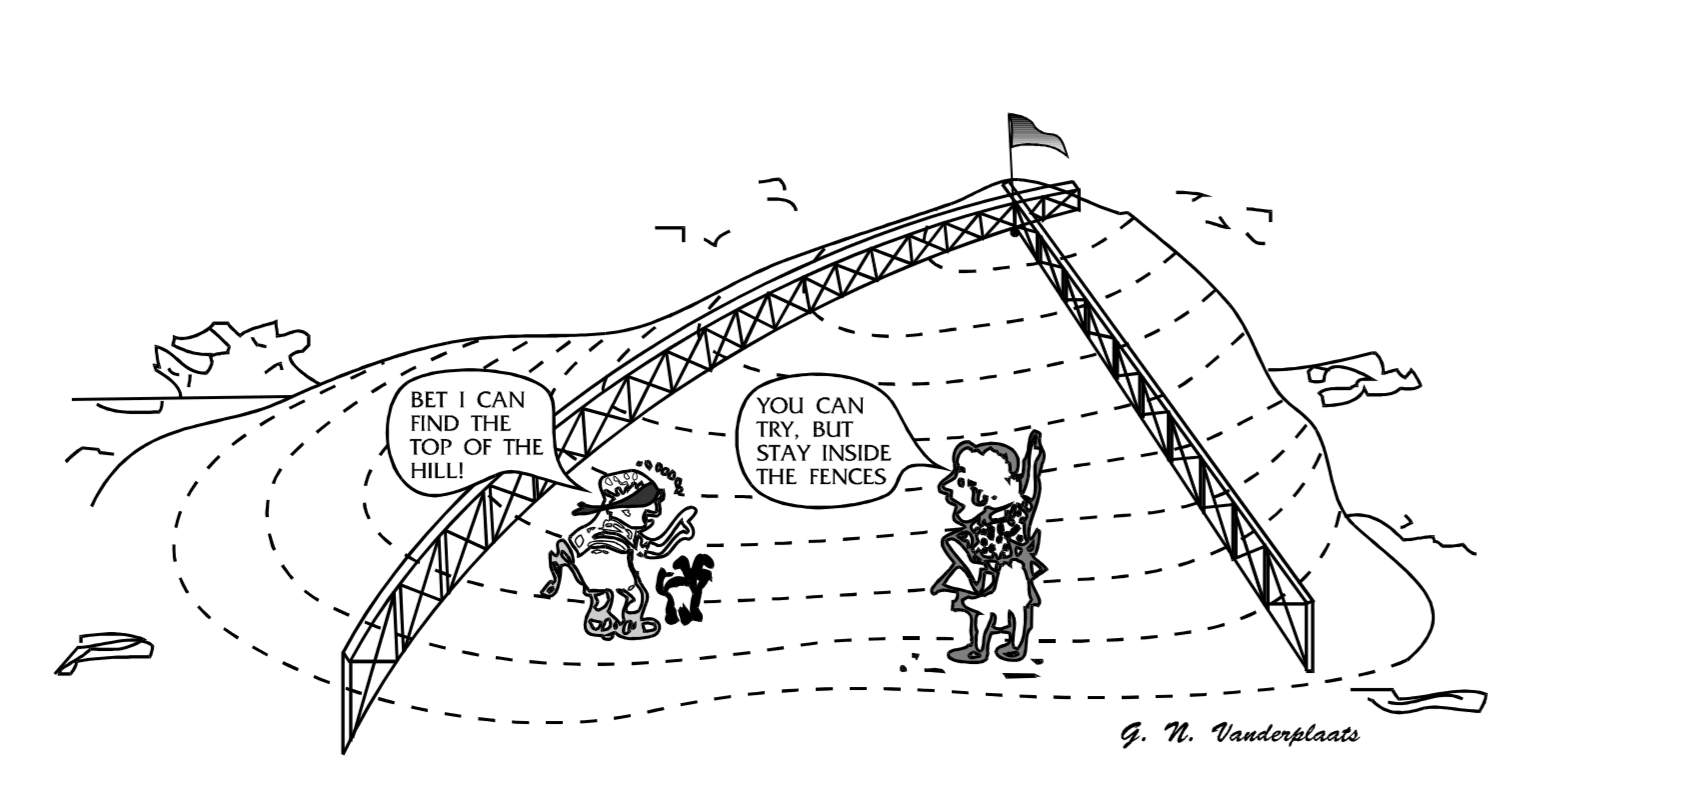
\includegraphics[width=1.0\textwidth]{figs/opt1.png}
%\end{figure}
%
%Cartoon by Dr. Gary Vanderplaats of \url{http://www.vrand.com/} some of these example problems and HW problems are from the DOT reference manual.
%\end{frame}
%
%\begin{frame}{Mathematical optimization formulation}
%Objective function:
%\begin{equation}
%\min F(\bm{x})
%\end{equation}
%Inequality constraints:
%\begin{equation}
%G(\bm{x}) \leq 0
%\end{equation}
%Variable constraints
%\begin{align}
%x_1^L \leq x_1 \leq x_1^U \\
%x_2^L \leq x_2 \leq x_2^U \\
%\cdots \\
%x_n^L \leq x_n \leq x_n^U 
%\end{align}
%\end{frame}
%
%\begin{frame}{Optimization in engineering: finding the best input}
%\begin{tikzpicture}[node distance=2cm]
%\node (in1) [startstop] {Input | $\bm{x}$};
%\node (pro1) [process, below of=in1] {CFD / FEA / MD / black box / $F(\bm{x})$};
%\node (dec1) [decision, below of=pro1, yshift=-0.5cm] {Best output?};
%\node (pro2b) [process, right of=dec1, xshift=2cm] {Try again};
%\node (stop) [startstop, below of=dec1] {Stop};
%%\draw [arrow] (start) -- (in1);
%\draw [arrow] (in1) -- (pro1);
%\draw [arrow] (pro1) -- (dec1);
%\draw [arrow] (dec1) -- node[anchor=south] {no} (pro2b);
%\draw [arrow] (pro2b) |- (pro1);
%\draw [arrow] (dec1) -- node[anchor=east] {yes} (stop);
%\draw [arrow] (dec1) -- (stop);
%\end{tikzpicture}
%\end{frame}
%
%\begin{frame}{scipy.optimize at a glance}
%\begin{itemize}
%\item local and global optimization algorithms
%\item gradient and stochastic
%\item constrainted and unconstrained algorithms 
%\end{itemize}
%\url{https://docs.scipy.org/doc/scipy/reference/tutorial/optimize.html}
%\url{https://docs.scipy.org/doc/scipy/reference/optimize.html}
%\end{frame}
%
%\begin{frame}{Unconstrained multivariate methods}
%\begin{table}
%\begin{tabular}{ll}
%\textbf{Method} & \textbf{Description}  \\
%\hline
%fmin & Minimize a function using the downhill simplex algorithm.\\
%fmin\_powell & Minimize a function using modified Powell’s method.\\
%fmin\_cg & Nonlinear conjugate gradient algorithm.\\
%fmin\_bfgs & Minimize a function using the BFGS algorithm.\\
%fmin\_ncg &	Minimization of a function using the Newton-CG method.\\
%\end{tabular}
%\end{table}
%\end{frame}
%
%\begin{frame}{Constrained multivariate methods}
%\begin{table}
%\begin{tabular}{ll}
%\textbf{Method} & \textbf{Description}  \\
%\hline
%fmin\_l\_bfgs\_b &	Minimize using the L-BFGS-B algorithm.\\
%fmin\_tnc & 	Minimize a function with truncated Newton algorithm.\\
%fmin\_cobyla &  	Constrained Optimization BY Linear Approximation.\\
%fmin\_slsqp &  	Minimize using Sequential Least SQuares Programming\\
%differential\_evolution & 	Finds the global minimum of a multivariate function.\\
%\end{tabular}
%\end{table}
%\end{frame}
%
%\begin{frame}{Global optimization methods}
%\begin{table}
%\begin{tabular}{ll}
%\textbf{Method} & \textbf{Description}  \\
%\hline
%basinhopping &	Global minimum using the basin-hopping algorithm\\
%brute & 	Minimize a function over a given range by brute force.\\
%differential\_evolution & 	Finds the global minimum of a multivariate function.\\
%\end{tabular}
%\end{table}
%\end{frame}
%
%\begin{frame}{Methods I like}
%\begin{table}
%\begin{tabular}{lll}
%\textbf{Method} & \textbf{My use} & \textbf{Pitfall}  \\
%\hline
%fmin\_bfgs  & local & local minima \\
%fmin\_l\_bfgs\_b  & bounded local & local minima \\
%fmin\_slsqp $\ast$ & Constrained local & Quadratic and local minima \\
%differential\_evolution & 	Global optimization & Number of function evaluations \\
%\end{tabular}
%\end{table}
%$\ast$ the only true constrained optimization algorithm...
%\end{frame}
%
%\begin{frame}{Optimizing engineering problems}
%\begin{itemize}
%\item optimization is a great design tool
%\item FEA/ CFD/ MD take a long time to evaluate
%\item can only afford a limited number of function evaluations
%\item there is no method that will work well on all problems (see No Free Lunch by Wolpert and Macready 1997)  \url{https://ti.arc.nasa.gov/m/profile/dhw/papers/78.pdf}
%\item Gradient based methods, non-gradient (stochastic) based methods, surrogate base methods, and various combinations
%\end{itemize}
%\end{frame}
%
%\begin{frame}{Gradient based methods}
%\begin{itemize}
%\item work well when you have an initial design
%\item guaranteed to find an optima (thought it might be a local one)
%\item work with a large number of design variables ($ n > 1000$) 
%\item make the most of your function evaluations
%\item deal with multiminima by running multiple optimization from different starting point
%\item function must be smooth and near continuous! 
%\end{itemize}
%\end{frame}
%
%\begin{frame}{Global optimization methods}
%\begin{itemize}
%\item large number of function evaluations (which is fine when you can afford it)
%\item stochastic/evolutionary methods not guaranteed to converge to a minima
%\item sometimes we just want to find the best solution
%\item functions can be discontinuous 
%\end{itemize}
%\end{frame} 
%
%\begin{frame}[fragile]{fmin\_bfgs basic gradient based method}
%\url{https://docs.scipy.org/doc/scipy/reference/generated/scipy.optimize.fmin_bfgs.html#scipy.optimize.fmin_bfgs}
%\begin{minted}
%{python}
%res = fmin_bfgs(f, x0, fprime=None, args=(), gtol=1e-05, 
%norm=inf, epsilon=1.4901161193847656e-08, maxiter=None, 
%full_output=0,  disp=1, retall=0, callback=None)
%\end{minted}
%\end{frame}
%
%\begin{frame}[fragile]{fmin\_l\_bfgs\_b constrained version of BFGS}
%\url{https://docs.scipy.org/doc/scipy/reference/generated/scipy.optimize.fmin_l_bfgs_b.html#scipy.optimize.fmin_l_bfgs_b}
%\begin{minted}
%{python}
%res = fmin_l_bfgs_b(func, x0, fprime=None, args=(), 
%approx_grad=0, bounds=None, m=10, factr=10000000.0, 
%pgtol=1e-05, epsilon=1e-08,  iprint=-1, maxfun=15000, 
%maxiter=15000, disp=None,   callback=None, maxls=20)
%\end{minted}
%\end{frame}
%
%\begin{frame}[fragile]{differential evolution}
%\url{https://docs.scipy.org/doc/scipy/reference/generated/scipy.optimize.differential_evolution.html#scipy.optimize.differential_evolution}
%\begin{minted}
%{python}
%res = differential_evolution(func, bounds, args=(), 
%strategy='best1bin', maxiter=1000, popsize=15, tol=0.01,
% mutation=(0.5, 1), recombination=0.7,  seed=None, 
% callback=None,  disp=False, polish=True,   
% init='latinhypercube', atol=0)
%\end{minted}
%\end{frame}
%
%\begin{frame}{differential evolution parameters}
%I really love all the feature with this algorithm... 
%\begin{itemize}
%\item strategy: the differential evolution strategy
%\item polish: if true a L-BFGS-B optimization is run with the optima found by differential evolution (This is a true meta-heuristic algorithm! - great global optimization) 
%\item init: by default the first generation is made with a latin hypercube sampling!
%\end{itemize}
%warning this could use a considerable number of function evaluations
%\end{frame}
%
%\begin{frame}{Example 1: non-linear regression with BFGS 1 of 3}
%Consider fitting a function
%\begin{equation}
%f(\bm{\beta}, x) = \frac{\beta_0 x}{\beta_1 + x}
%\end{equation}
%in this case $\bm{\beta}$ are the design variables and x are the data points. 
%
%For this example I'm going to fit this function to some data points. 
%
%In most cases you won't know the exact beta parameters that the data comes from, but it makes for an easy example to know the solution.
%
%\end{frame}
%
%\begin{frame}[fragile]{Example 1: non-linear regression with BFGS 2 of 3}
%\begin{minted}
%{python}
%import numpy as np
%import matplotlib.pyplot as plt
%from scipy import optimize
%
%# generate some data from known beta values
%x = np.linspace(0,10,30)
%beta0 = 2.7
%beta1 = 1.3
%y = (beta0*x)/(beta1+x)
%
%# determine beta by minimizing the mean residual error
%def my_func(X):
%    yHat = (X[0]*x)/(X[1]+x)
%    resid = yHat - y
%    return np.mean(np.abs(resid))
%\end{minted}
%\end{frame}
%
%\begin{frame}[fragile]{Example 1: non-linear regression with BFGS 3 of 3}
%\begin{minted}
%{python}
%# peform the optimization with bfgs
%x0 = [3.0, 3.0] # initial guess
%res = optimize.fmin_bfgs(my_func, x0, full_output=True) 
%
%plt.figure()
%plt.plot(x,y,'o')
%beta = res[0] # these are the resulting beta parameters
%# plot the resulting curve
%plt.plot(x,(beta[0]*x)/(beta[1]+x))
%plt.show()
%\end{minted}
%\end{frame}
%
%\begin{frame}[fragile]{Example 2: constrained optimization 1 of 4}
%Minimize
%\begin{equation}
%F(\bm{x}) = (x_0 + x_1)^2 + (x_1 + x_2)^2
%\end{equation}
%subject to
%\begin{equation}
%h_0 = x_0 + 2x_1 + 3x_2 - 1 = 0
%\end{equation}
%from the initial design point of
%\begin{equation}
%\bm{x_0} = [-4.0, 1.0, 2.0]
%\end{equation}
%\textbf{Note}: You always set up your equality constraints equal to 0!
%\end{frame}
%
%\begin{frame}[fragile]{Example 2: constrained optimization 2 of 4}
%\begin{minted}
%{python}
%# objective function
%def func(X):
%    F = (X[0]+X[1])**2 + (X[1]+X[2])**2
%    return F
%# equality constraint
%def f_con(X):
%    G = X[0] + 2.0*X[1] + 3.0*X[2] - 1.0
%    return G
%# initial design point
%x0 = np.array([-4.0, 1.0, 2.0])    
%res = optimize.fmin_slsqp(func, x0, f_eqcons=f_con,
%    iter=1000, acc=1e-06, disp=True, full_output=True)
%\end{minted}
%\end{frame}
%
%\begin{frame}[fragile]{Example 2: constrained optimization 3 of 4}
%Minimize
%\begin{equation}
%F(\bm{x}) = (x_0 + x_1)^2 + (x_1 + x_2)^2
%\end{equation}
%subject to an alternative inequality constraints
%\begin{equation}
%g_0 = x_0 + 2x_1 + 3x_2 - 1 \leq 0
%\end{equation}
%\begin{equation}
%g_1 = -g_0 \leq 0
%\end{equation}
%from the initial design point of
%\begin{equation}
%\bm{x_0} = [-4.0, 1.0, 2.0]
%\end{equation}
%\textbf{Note}: You always set up your inequality constraints less than or equal to zero!
%\end{frame}
%
%\begin{frame}[fragile]{Example 2: constrained optimization 4 of 4}
%\begin{minted}
%{python}
%# objective function
%def func(X):
%    F = (X[0]+X[1])**2 + (X[1]+X[2])**2
%    return F
%# inequality constraint
%# note slsqp handles Gradient contraints as >= 0 and not <=0
%# so for this case i have G >= 0 and -G > = 0
%# don't ask me why... I have no clue why
%def f_con1(X):
%    G = X[0] + 2.0*X[1] + 3.0*X[2] - 1.0
%    return G, -G
%# initial design point
%x0 = np.array([-4.0, 1.0, 2.0])    
%res = optimize.fmin_slsqp(func, x0, f_ieqcons=f_con1, 
%    iter=1000, acc=1e-06, disp=True, full_output=True)
%\end{minted}
%\end{frame}
%
%\begin{frame}{Example 3: Global optimization of the Adjiman function}
%Minimize
%\begin{equation}
%f( \bm{x} ) = \cos (x_0) \sin (x_1) - \frac{x_0}{x_1^2 +1}
%\end{equation}
%on the domain
%\begin{equation}
%-10 \leq x_0 \leq 10
%\end{equation}
%\begin{equation}
%-10 \leq x_1 \leq 10
%\end{equation}
%\end{frame}
%
%\begin{frame}[fragile]{Example 3: Global optimization of the Adjiman function}
%Differential evolution works well on this multimodal problem.
%\begin{minted}
%{python}
%# objective function
%def adjiman(x):
%    F = np.cos(x[0])*np.sin(x[1]) - ((x[0])/(x[1]**2 +1.0))
%    return F
%    
%# optimization bounds 
%bounds = ((-10.0,10.0),
%          (-10.0,10.0))    
%# run differential evolution          
%res = optimize.differential_evolution(adjiman, bounds, 
%    maxiter=1000, popsize=50, disp=True)
%\end{minted}
%\end{frame}
%
%\begin{frame}{Example 3: Global optimization of the Adjiman function}
%\begin{figure}
%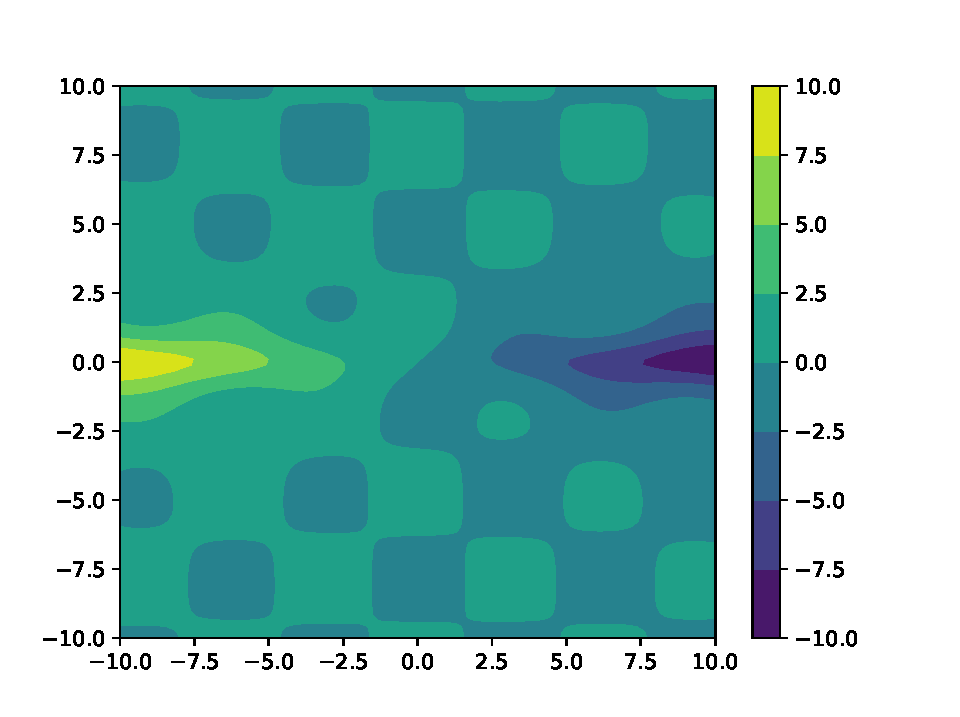
\includegraphics[width=1.0\textwidth]{figs/adjiman.pdf}
%\end{figure}
%\end{frame}
%
%\begin{frame}[fragile]{Example 3: Global optimization of the Adjiman function}
%Issues with L-BFGS-B
%\begin{minted}
%{python}
%# objective function
%def adjiman(x):
%    F = np.cos(x[0])*np.sin(x[1]) - ((x[0])/(x[1]**2 +1.0))
%    return F
%    
%# optimization bounds 
%bounds = ((-10.0,10.0),
%          (-10.0,10.0))    
%          
%# this l bfgs b won't find the optimum
%res2 = optimize.fmin_l_bfgs_b(adjiman, (-2,-2), 
%    approx_grad=True, bounds=bounds)
%
%# however this l bfgs b will
%res3 = optimize.fmin_l_bfgs_b(adjiman, (2,2), 
%    approx_grad=True, bounds=bounds)
%\end{minted}
%\end{frame}



\end{document}
